\chapter{Result Analysis}
\section{Robot Movement}
The robot movement in various directions was performed by pressing the a, w, s, d keys on the keyboard. The robot reacted spontaneously. This was accomplished with the help of wifi and delay less transfer  of data. Upon pressing of the keys the respective robot movement in different directions was observed. In addition to this we demonstrated the working of the motors by the means of LED bulb s and a table to showed the multidirectional movement.
\begin{figure}[h]
\centering
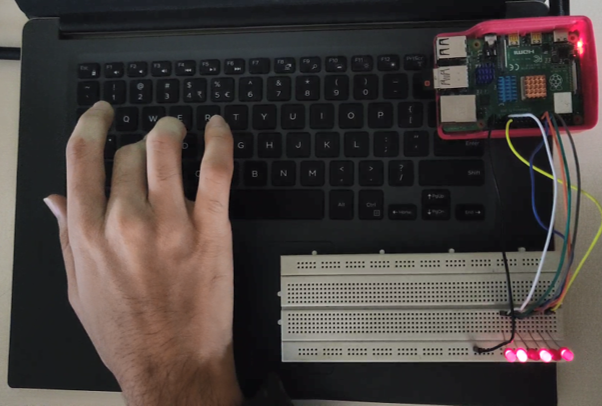
\includegraphics[scale=0.8]{led.png}
\caption{Working of motor using LEDs}
\end{figure}
\newpage
\section{Live Feed Capture}
The camera connected to the raspberry pi gave instant camera feed without any delay. This was reflected on the websites that we developed .It was observed that the camera quality was good and hence clear images were obtained.
\begin{figure}[h]
\centering
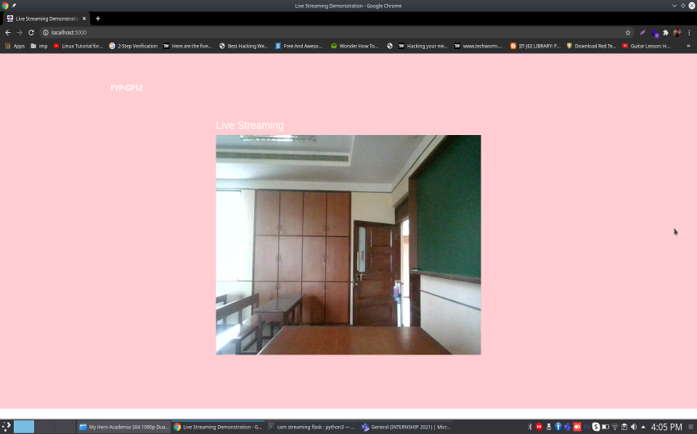
\includegraphics[scale=0.8]{webpage.png}
\caption{Local Live feed on Webpage}
\end{figure}